\documentclass[11pt,a4paper]{article}
\usepackage[margin=2.2cm]{geometry}
\usepackage{graphicx}
\usepackage{booktabs}
\usepackage{float}
\usepackage{amsmath}
\usepackage{xcolor}
\usepackage{microtype}
\usepackage{fancyvrb}
\usepackage[colorlinks=true,linkcolor=blue!50!black,urlcolor=blue!60!black]{hyperref}
\makeatletter\g@addto@macro{\UrlBreaks}{\UrlOrds}\makeatother % allow long URLs to wrap
\setlength{\parskip}{0.5em}
\setlength{\parindent}{0pt}

% Figures: a W&B screenshot in figures/wandb/<name>.png replaces the local rendering.
\newcommand{\wbfig}[3]{%
  \IfFileExists{figures/wandb/#1.png}%
    {\includegraphics[width=#3\linewidth]{figures/wandb/#1.png}}%
    {\includegraphics[width=#3\linewidth]{figures/#2.png}}}

\newcommand{\repo}{\url{https://github.com/gb0x11/CS6886W-Assignment-1}}
\newcommand{\wbproject}{\url{https://forge.coreweave.com/wandb/cs25m508-indian-institute-of-technology/cs6886w-vgg6-cifar10}}
\newcommand{\wbreport}{\href{https://forge.coreweave.com/cs25m508-indian-institute-of-technology/cs6886w-vgg6-cifar10/reports/CS6886W-A1:-VGG6-on-CIFAR-10-(Question-3-plots)--VmlldzoxODE3NjQ4Mw==}{W\&B report: Question 3 plots}}

\newcommand{\NumRuns}{39}
\newcommand{\BestVal}{86.36}
\newcommand{\BestTest}{85.72}
\newcommand{\BestEpoch}{100}
\newcommand{\BestName}{act\_relu\_bs\_64\_opt\_nadam\_lr\_0.003\_wd\_0.0005\_ep\_100\_bn\_True}

\providecommand{\ParallelDetail}{}

\begin{document}

\begin{center}
{\LARGE\bfseries CS6886W: Systems Engineering for Deep Learning}\\[4pt]
{\Large Assignment 1: VGG6 on CIFAR-10}\\[10pt]
{\large Gowtham B \quad (CS25M508)}\\[6pt]
GitHub repository: \repo\\
W\&B project: \wbproject\\
\wbreport
\end{center}

\section*{Experimental setup (common to all questions)}

\textbf{Model.} VGG6 exactly as in the course template: conv(64), conv(64), max-pool, conv(128), conv(128), max-pool, each conv $3\times3$ with padding 1, optionally followed by BatchNorm, then the activation; global average pooling and one linear layer $128\to10$. The network has 262{,}218 parameters. Only the activation function and the use of BatchNorm are changed between runs.

\textbf{Data split.} The 50{,}000 CIFAR-10 training images are split (fixed seed) into 45{,}000 for training and 5{,}000 for \emph{validation}. The validation split is used for model selection (``best validation accuracy''); the official 10{,}000 test images are only used to report the final test accuracy of the checkpoint with the best validation accuracy.

\textbf{Training.} Cross-entropy loss, cosine learning-rate decay to zero over the run (per step), weight decay $5\times10^{-4}$ (L2), seed 42, Apple M1 Pro GPU (PyTorch 2.14.1, MPS backend), about 18\,s per epoch. Every run logs \texttt{train\_loss}, \texttt{train\_acc}, \texttt{val\_loss}, \texttt{val\_acc} and \texttt{lr} once per epoch to W\&B.

\textbf{Baseline for Question 2.} Each experiment family changes exactly one setting of a shared baseline: ReLU, BatchNorm on, SGD with momentum 0.9, learning rate 0.05, batch size 128, 20 epochs. In total \NumRuns{} runs were trained.

%=====================================================================
\section*{Question 1: Training baseline}

\subsection*{(a) Data preparation and transforms}

\begin{center}
\small
\begin{tabular}{lll}
\toprule
Split & Transform (in order) & Parameters \\
\midrule
Train & RandomCrop & $32\times32$ crop after zero-padding 4 px per side \\
      & RandomHorizontalFlip & $p=0.5$ \\
      & ToTensor & uint8 $[0,255]\to$ float $[0,1]$ \\
      & Normalize & mean $(0.4914, 0.4822, 0.4465)$, std $(0.2023, 0.1994, 0.2010)$ \\
      & Cutout & one $16\times16$ square set to 0 (= channel mean), random centre \\
\midrule
Val / test & ToTensor, Normalize & same mean / std, no augmentation \\
\bottomrule
\end{tabular}
\end{center}

The mean and standard deviation are the per-channel statistics of the CIFAR-10 training set, so the normalised inputs have roughly zero mean and unit variance, which keeps the first layer's activations well scaled for every activation function. Random crops (translations of up to $\pm4$ pixels) and horizontal flips encode the invariances of natural images; Cutout forces the network to use several parts of the object instead of a single discriminative patch. These are the transforms of the course template. To remove the CPU data-loading bottleneck the whole dataset is stored on the GPU and the identical operations are applied there per mini-batch (\texttt{vgg6/data.py}).

\subsection*{(b) Chosen configuration}

The baseline trained for Question 1 is the best configuration found in Question 2 (it is also the answer to Question 4):

\begin{center}
\begin{tabular}{ll}
\toprule
Setting & Value \\
\midrule
Activation / BatchNorm & ReLU / on \\
Optimizer & Nadam ($\beta_1=0.9$, $\beta_2=0.999$), learning rate $3\times10^{-3}$ \\
Schedule & cosine decay to 0 over all steps, no warm-up \\
Weight decay & $5\times10^{-4}$ (L2) \\
Batch size / epochs & 64 / 100 \\
Augmentation & crop + flip + Cutout(16), Question 1(a) \\
Seed & 42 \\
\bottomrule
\end{tabular}
\end{center}

\textbf{Why this configuration.} Question 2(b) showed Nadam with lr $3\times10^{-3}$ to be the best and fastest optimizer (84.74\% after 20 epochs, ahead of Nesterov SGD at 84.14\%); a larger rate (0.006) was worse (83.38\%), and with Nadam ReLU beat GELU (84.74 vs.\ 84.02\%). Question 2(a) showed ReLU and GELU to be the best activations. Question 2(c) showed that a smaller batch (64 instead of 128) improves accuracy at a moderate cost in time, and that accuracy keeps increasing with the number of epochs without over-fitting (85.9\% at 40 epochs with plain momentum SGD), so the final model is trained for 100 epochs.

\subsection*{(c) Final test accuracy and curves}

The checkpoint with the best validation accuracy (\BestVal\% at epoch \BestEpoch) reaches a \textbf{final test top-1 accuracy of \BestTest\%} on the 10{,}000 CIFAR-10 test images. Figure~\ref{fig:best} shows its loss and accuracy curves.

\begin{figure}[H]
\centering
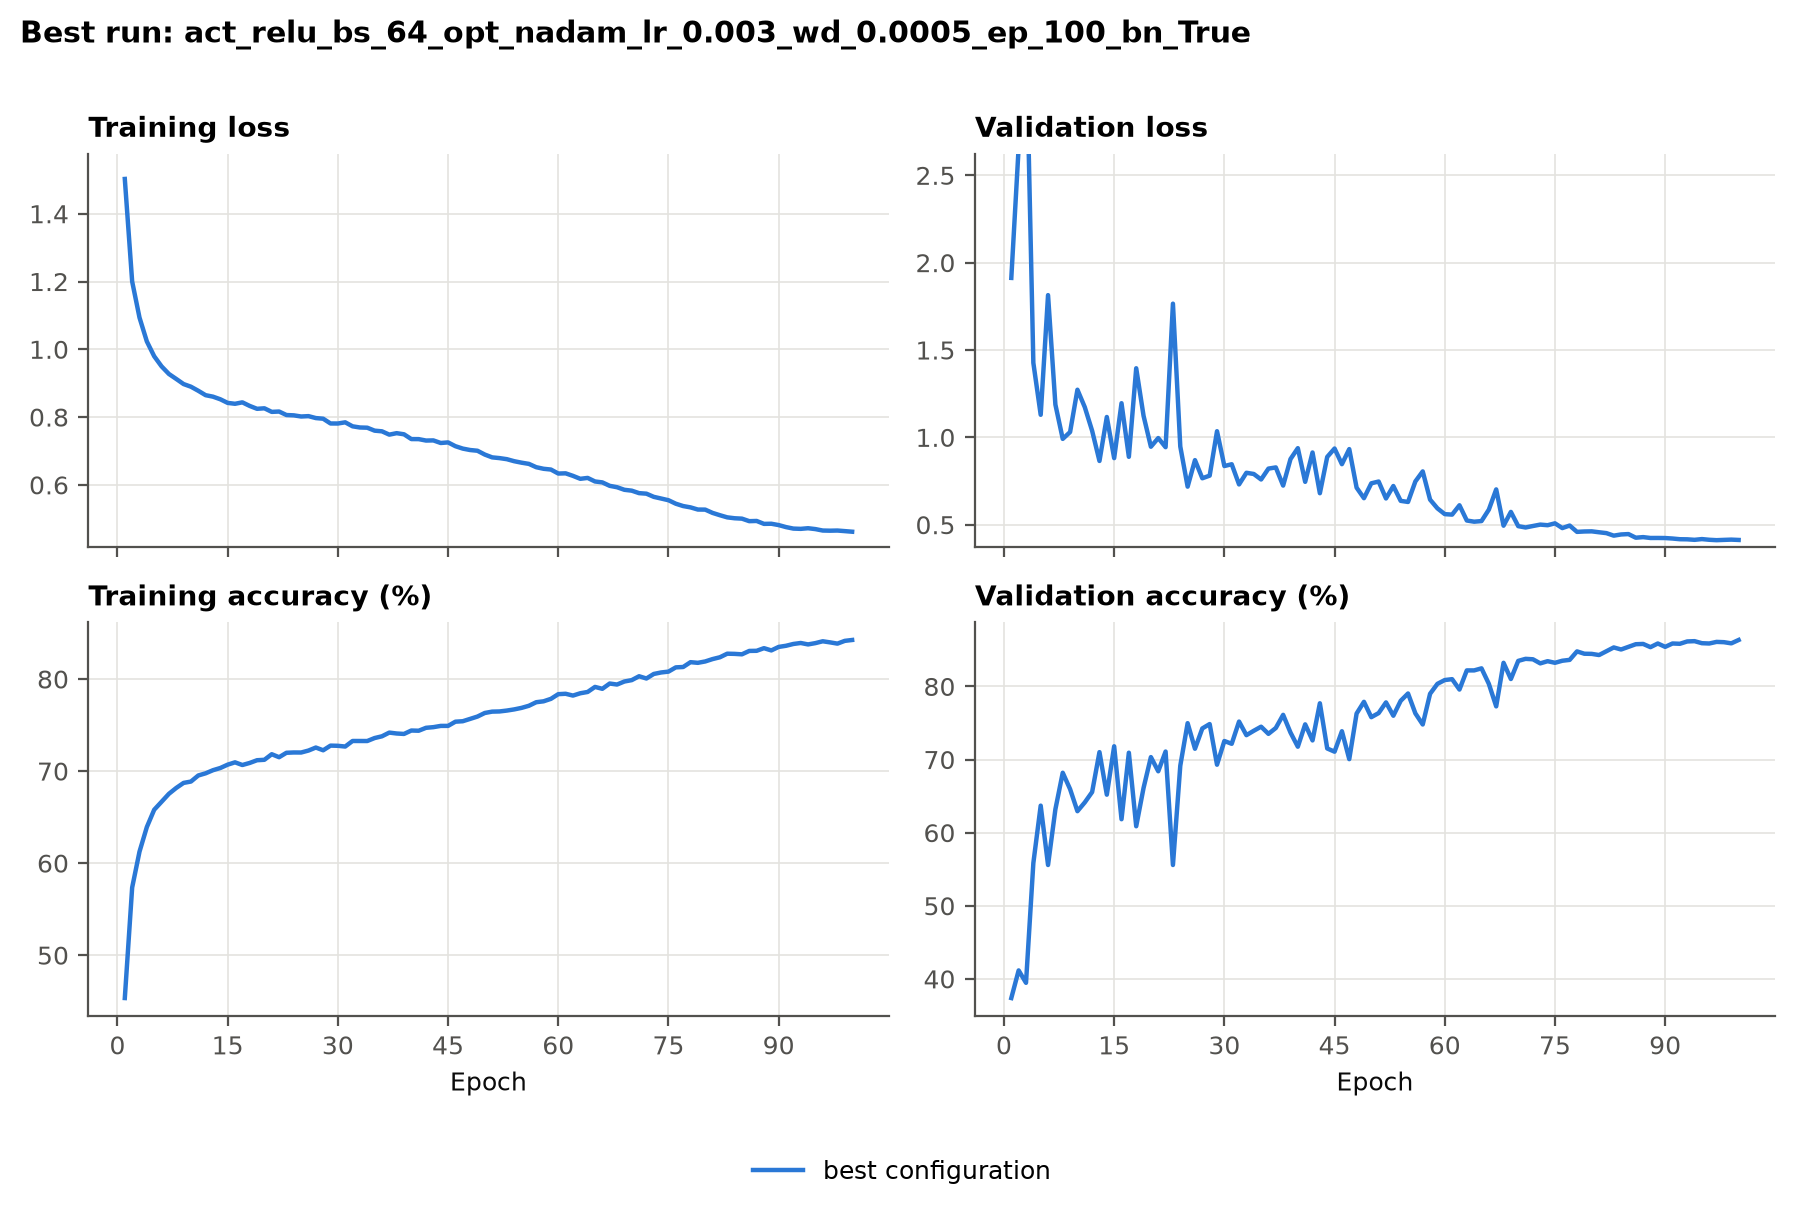
\includegraphics[width=0.78\linewidth]{figures/best_run.png}
\caption{Loss and accuracy curves of the best configuration. Training metrics are measured on the augmented mini-batches during the epoch, which is why training accuracy sits below validation accuracy.}
\label{fig:best}
\end{figure}

%=====================================================================
\section*{Question 2: Model performance on different configurations}

\subsection*{(a) Activation functions}

All five activations were trained with the baseline (BatchNorm on, momentum SGD, lr 0.05, 20 epochs). \IfFileExists{tables/activation_nobn.tex}{To separate the effect of the activation from that of BatchNorm, the same five were also trained without BatchNorm (lr 0.01, since the plain network diverges at 0.05).}{}

\begin{center}
\begin{tabular}{lrrrrr}
\toprule
Activation & Best val (\%) & Test (\%) & Best ep. & Ep. to 70\% & Final train (\%) \\
\midrule
relu & \textbf{83.16} & 81.66 & 19 & 8 & 79.82 \\
sigmoid & 59.92 & 59.50 & 20 & never & 57.21 \\
tanh & 70.48 & 70.23 & 20 & 19 & 67.19 \\
silu & 80.62 & 80.10 & 20 & 10 & 77.02 \\
gelu & 82.98 & 81.53 & 19 & 8 & 79.24 \\
\bottomrule
\end{tabular}

\end{center}
\IfFileExists{tables/activation_nobn.tex}{\begin{center}\textit{Without BatchNorm:}\\[2pt]\input{tables/activation_nobn.tex}\end{center}}{}

\begin{figure}[H]
\centering
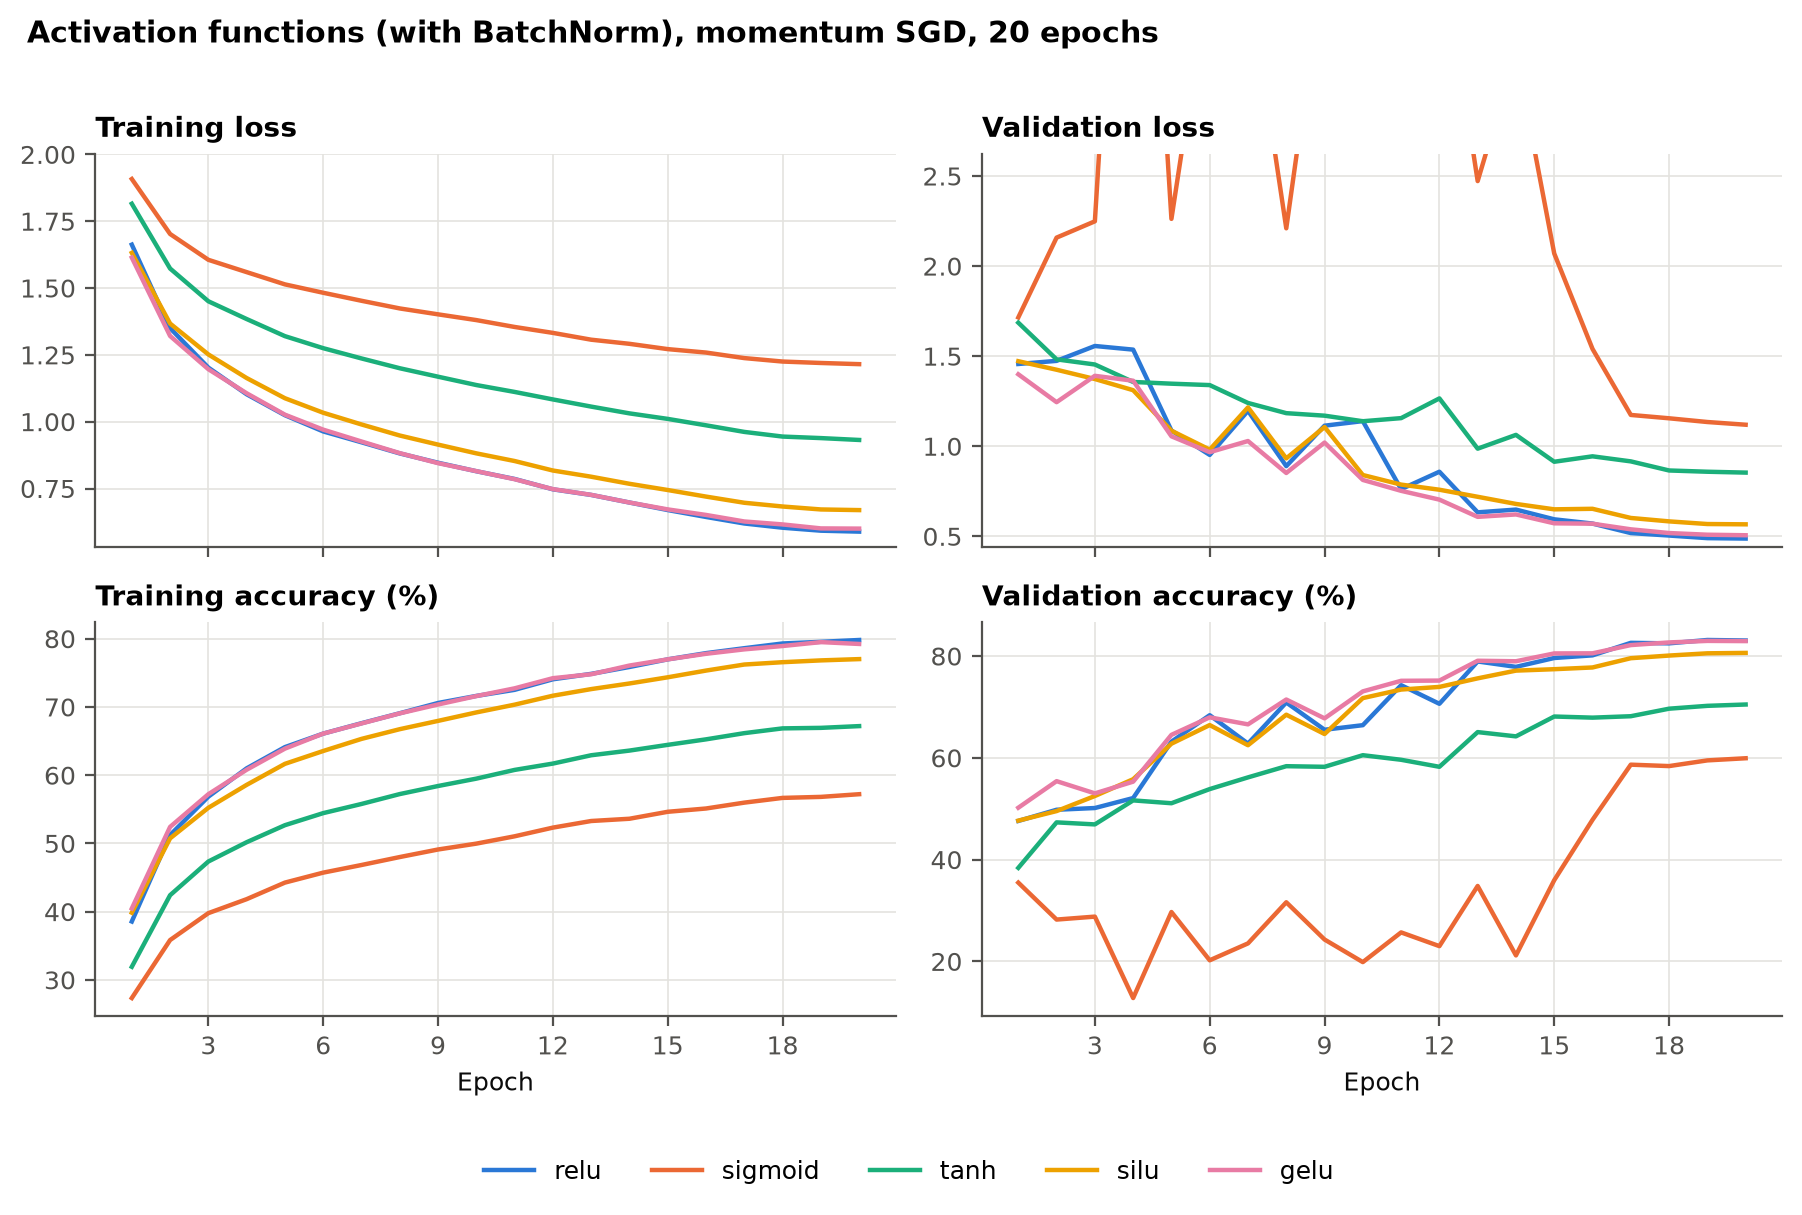
\includegraphics[width=0.92\linewidth]{figures/activation.png}
\caption{Activation functions with BatchNorm (momentum SGD, lr 0.05, 20 epochs).}
\end{figure}

\textbf{How performance changes.}
\begin{itemize}
\item \textbf{ReLU (83.16\%) and GELU (82.98\%) are best and practically tied}; the 0.2-point gap is within run-to-run noise. Both are non-saturating for positive inputs, so the gradient passes through each layer with slope close to 1 and all four conv layers learn quickly (70\% validation accuracy after 8 epochs).
\item \textbf{SiLU is close behind (80.62\%)}. It is also non-saturating, but its gate is softer than GELU's: SiLU is $x\,\sigma(x)$ while GELU is approximately $x\,\sigma(1.702x)$, so SiLU switches from ``off'' to ``linear'' over a range about 1.7 times wider and dips further below zero (minimum $-0.28$ vs.\ $-0.17$). With BatchNorm-normalised inputs a larger share of units therefore sit in the soft, nearly linear zone, which plausibly explains why it learned a little more slowly (70\% after 10 instead of 8 epochs) and ended about 2.5 points lower. With a single seed per setting, part of this gap may also be noise.
\item \textbf{Tanh (70.48\%) and sigmoid (59.92\%) are clearly worse.} Both saturate: their derivatives vanish for $|x|>2$, and the sigmoid derivative is at most 0.25, so the gradient shrinks by at least $4\times$ per layer. After BatchNorm the pre-activations are roughly $\mathcal N(0,1)$, which for tanh and sigmoid falls mostly into their nearly linear central region, so the network also behaves more like a linear model and has less useful non-linearity. Tanh is zero-centred with slope 1 at the origin and does much better than sigmoid, whose outputs are all positive (mean $\approx0.5$), which biases the next layer's gradients.
\item \textbf{Stability.} The sigmoid run's validation accuracy is very erratic (it dropped to 19.9\% at epoch 10 before recovering) while its training loss decreased smoothly, a sign that the BatchNorm running statistics used at evaluation time do not match the batch statistics seen in training for this activation at a high learning rate. The ReLU-family runs only show the usual high-learning-rate oscillations, which disappear as the cosine schedule anneals the learning rate.
\end{itemize}

\subsection*{(b) Optimizers}

A single shared learning rate would favour either the SGD family or the adaptive family, so each optimizer was run at three learning rates around its usual default (ReLU, BatchNorm, batch 128, 20 epochs, cosine decay, L2 weight decay $5\times10^{-4}$). ``SGD (plain)'' has no momentum; ``SGD + momentum'' (heavy ball, $\beta=0.9$) comes from the learning-rate study of Question~2(c).

\begin{center}
\small
\begin{tabular}{lrrrrr}
\toprule
Optimizer, learning rate & Best val (\%) & Test (\%) & Best ep. & Ep. to 70\% & Final train (\%) \\
\midrule
SGD (plain), lr=0.05 & 70.68 & 69.47 & 20 & 17 & 67.13 \\
SGD (plain), lr=0.1 & 75.66 & 74.78 & 19 & 14 & 71.74 \\
SGD (plain), lr=0.2 & 79.16 & 77.79 & 19 & 11 & 75.30 \\
Nesterov SGD, lr=0.01 & 75.90 & 74.59 & 18 & 13 & 72.21 \\
Nesterov SGD, lr=0.05 & 83.60 & 82.60 & 20 & 8 & 80.48 \\
Nesterov SGD, lr=0.1 & 84.14 & 83.97 & 20 & 8 & 81.47 \\
Adam, lr=0.0003 & 74.08 & 73.00 & 20 & 13 & 70.39 \\
Adam, lr=0.001 & 81.68 & 80.90 & 18 & 10 & 78.40 \\
Adam, lr=0.003 & 84.00 & 83.72 & 20 & 8 & 81.22 \\
Adagrad, lr=0.003 & 64.58 & 63.80 & 15 & never & 61.76 \\
Adagrad, lr=0.01 & 74.54 & 73.29 & 18 & 11 & 70.38 \\
Adagrad, lr=0.03 & 79.82 & 79.09 & 19 & 10 & 76.05 \\
RMSprop, lr=0.0001 & 63.84 & 63.34 & 20 & never & 61.03 \\
RMSprop, lr=0.0003 & 74.26 & 73.07 & 20 & 14 & 70.51 \\
RMSprop, lr=0.001 & 81.24 & 80.45 & 20 & 10 & 77.78 \\
Nadam, lr=0.0003 & 74.16 & 72.83 & 19 & 13 & 70.41 \\
Nadam, lr=0.001 & 81.70 & 81.13 & 20 & 11 & 78.67 \\
Nadam, lr=0.003 & \textbf{84.74} & 84.92 & 20 & 7 & 82.41 \\
SGD + momentum, lr=0.005 & 70.98 & 70.00 & 19 & 15 & 67.50 \\
SGD + momentum, lr=0.01 & 75.76 & 74.44 & 19 & 13 & 71.47 \\
SGD + momentum, lr=0.05 & 83.16 & 81.66 & 19 & 8 & 79.82 \\
SGD + momentum, lr=0.1 & 82.72 & 83.29 & 20 & 11 & 80.98 \\
SGD + momentum, lr=0.2 & 83.74 & 83.51 & 20 & 13 & 81.01 \\
\bottomrule
\end{tabular}

\end{center}

\begin{figure}[H]
\centering
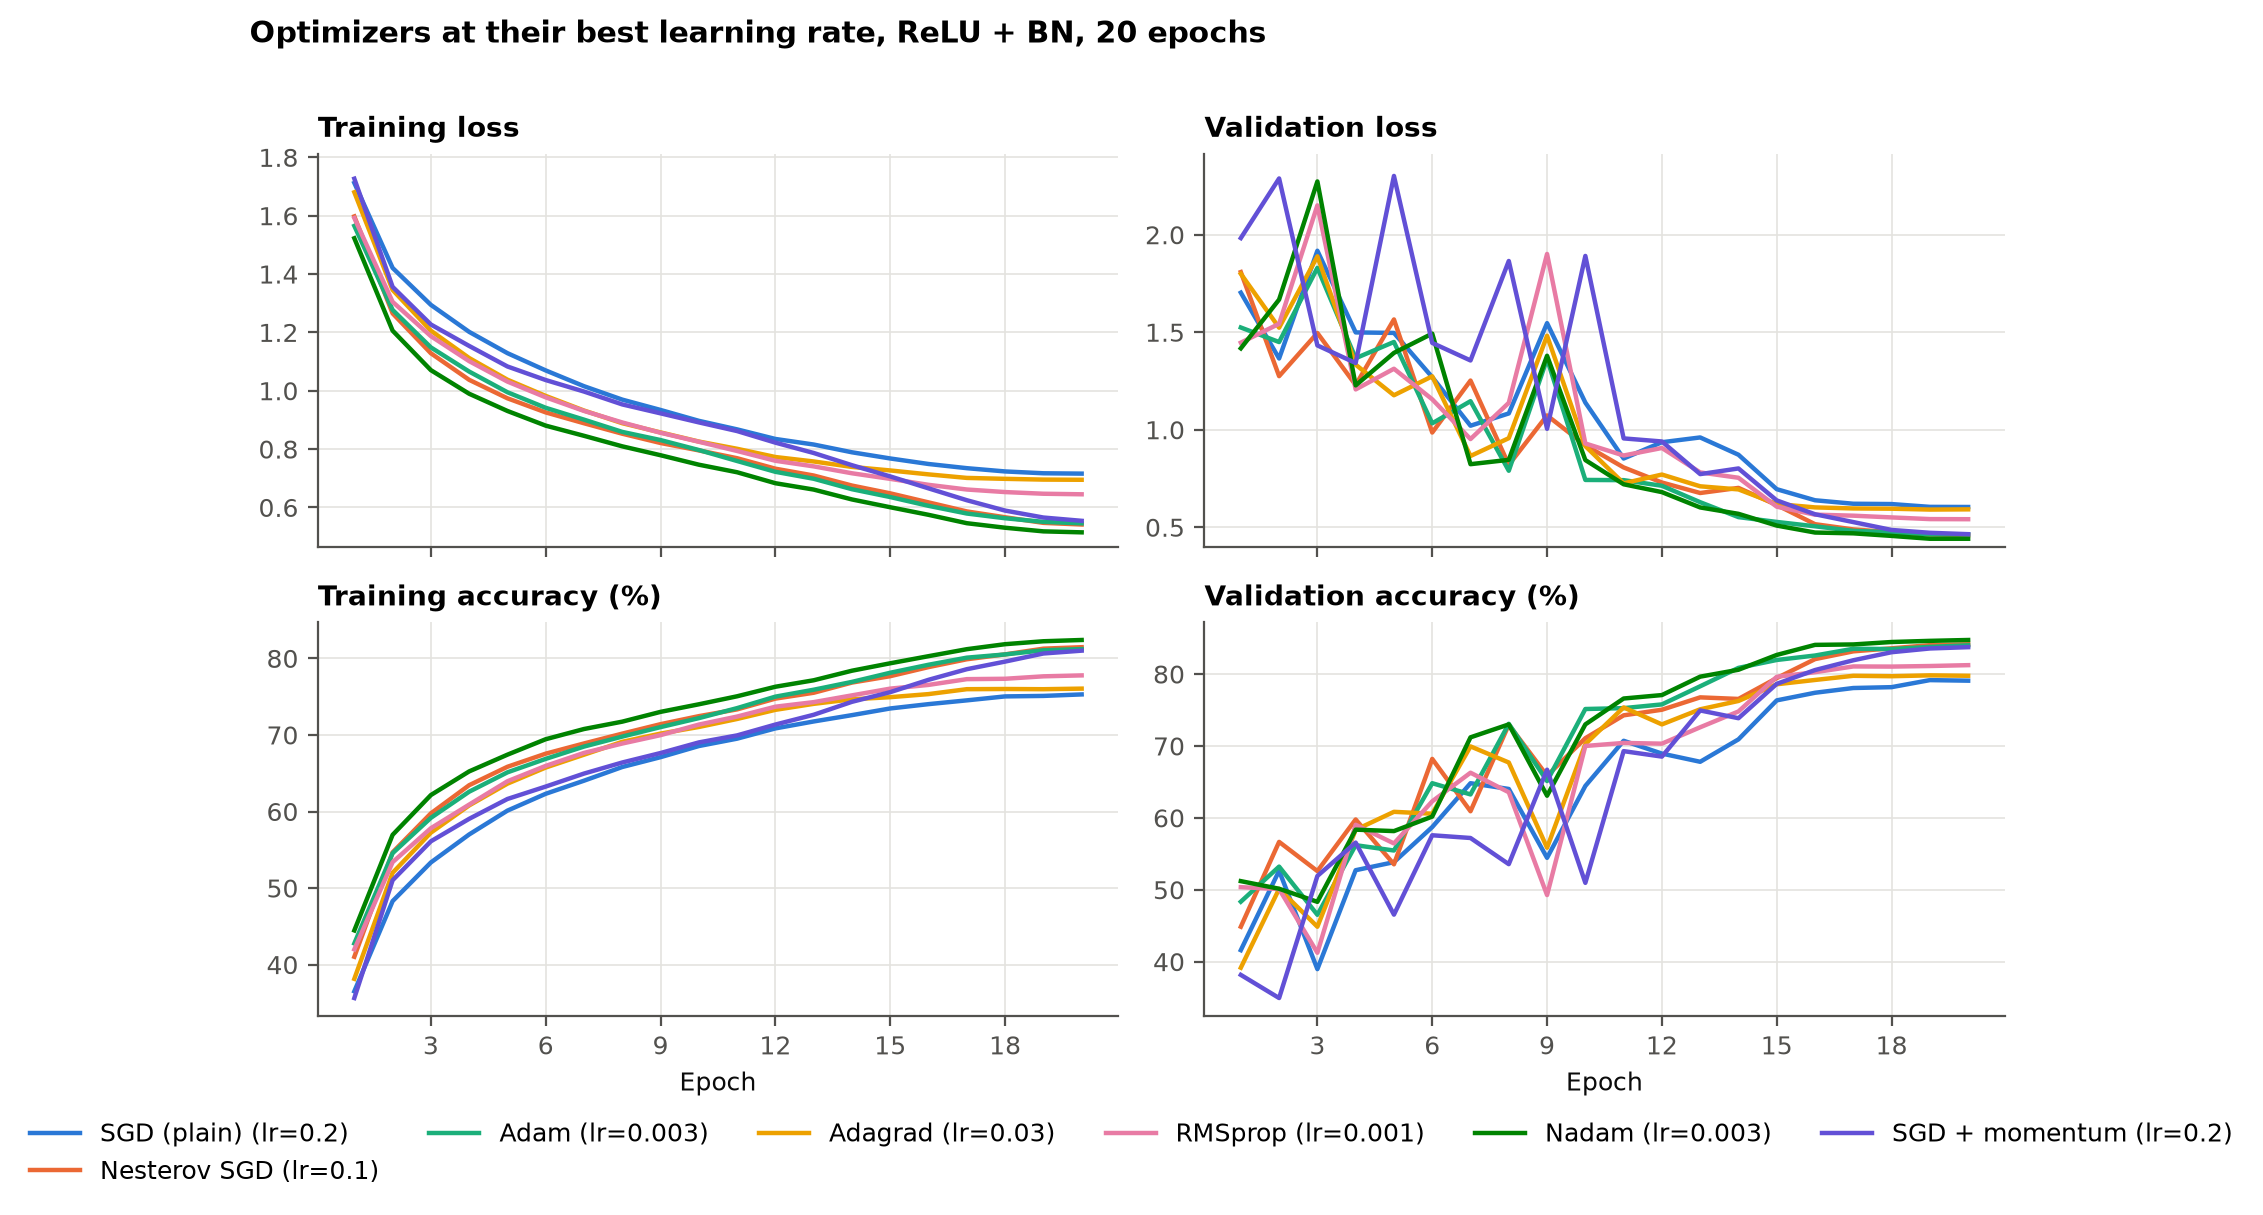
\includegraphics[width=0.92\linewidth]{figures/optimizer.png}
\caption{Each optimizer at its best learning rate.}
\end{figure}

\begin{figure}[H]
\centering
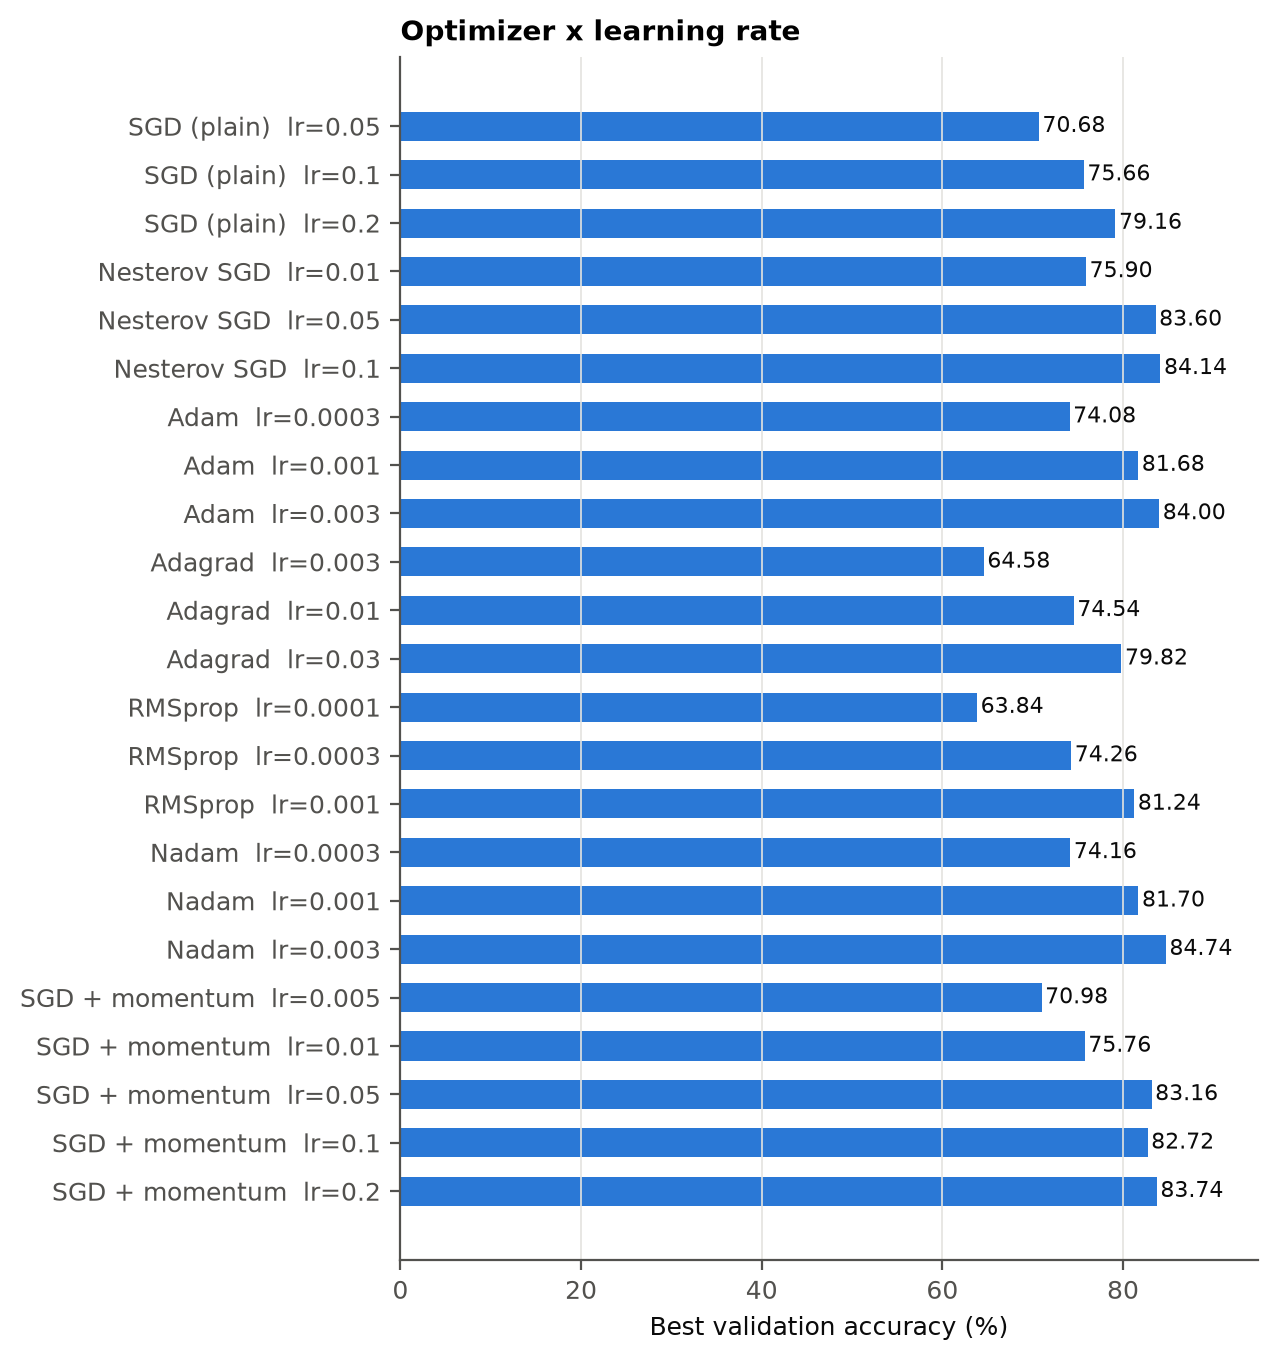
\includegraphics[width=0.62\linewidth]{figures/optimizer_lr_bars.png}
\caption{Best validation accuracy for every optimizer and learning rate.}
\end{figure}

\textbf{How each optimizer behaves.} Let $g_t$ be the mini-batch gradient and $\eta$ the learning rate.
\begin{itemize}
\item \textbf{SGD (plain):} $w \leftarrow w-\eta g_t$. Every step uses only the current noisy gradient, so progress along the low-curvature directions of the loss is slow. It is the slowest optimizer (70\% validation accuracy only after 11 to 17 epochs) and the only one that stays below 80\% after 20 epochs, even at lr 0.2. Accuracy keeps rising with the learning rate (70.7, 75.7, 79.2\%), showing that it is step-size limited.
\item \textbf{SGD + momentum:} $v\leftarrow\beta v+g_t$, $w\leftarrow w-\eta v$. Momentum averages gradients over about $1/(1-\beta)=10$ steps, which cancels noise and amplifies consistent directions by roughly $10\times$. At lr 0.05 it reaches 83.2\%, beating plain SGD at a 4$\times$ larger learning rate.
\item \textbf{Nesterov SGD:} the gradient is evaluated at the look-ahead point $w-\eta\beta v$, which corrects the step before it overshoots. At equal learning rate it is slightly better than heavy-ball momentum (83.6 vs.\ 83.2\% at lr 0.05), and it remains stable at lr 0.1 (84.1\%).
\item \textbf{Adagrad:} divides each coordinate's step by $\sqrt{\sum_{s\le t} g_s^2}$. Because the sum only grows, the effective learning rate decays monotonically; parameters with large early gradients practically stop learning. It needs a large learning rate (0.03) and still lags (79.8\%); at lr 0.003 the training loss plateaus at 1.11 and validation accuracy at 64.6\%.
\item \textbf{RMSprop:} replaces Adagrad's sum by an exponential moving average of $g^2$ (decay 0.99), so the step size no longer vanishes. It has no momentum and no bias correction here. It does much better than Adagrad (81.2\% at lr $10^{-3}$) but is very sensitive to the learning rate (63.8\% at $10^{-4}$).
\item \textbf{Adam:} momentum on $g$ (first moment) plus RMSprop-style scaling (second moment), both bias-corrected. Per-parameter step sizes make it fast early on; with lr $3\times10^{-3}$ it reaches 84.0\%, on par with Nesterov SGD. Like every method here it improved monotonically with the learning rate within the tested range.
\item \textbf{Nadam:} Adam with a Nesterov look-ahead on the first moment. It is the \textbf{fastest} (70\% after 7 epochs) and the \textbf{best} optimizer in this study: 84.74\% validation and 84.92\% test accuracy at lr $3\times10^{-3}$. At $3\times10^{-4}$ and $10^{-3}$ it matches Adam almost exactly, so its advantage appears when the step is large, where the look-ahead reduces overshoot.
\end{itemize}

\textbf{Differences and general observations.}
(1) Adaptive methods (Adam, Nadam, RMSprop) work at learning rates about 30 to 100 times smaller than SGD because their step is normalised by the gradient magnitude; comparing optimizers at one shared learning rate would therefore be meaningless.
(2) Momentum (heavy ball, Nesterov, or the first moment of Adam and Nadam) is the single most important ingredient: the four methods with momentum reach 83 to 85\%, the three without it (plain SGD, Adagrad, RMSprop) 79 to 81\%.
(3) Larger learning rates make the mid-training validation curves noisy (standard deviation of validation accuracy over epochs 5 to 15 of about 8 points at the largest learning rates vs.\ 2 to 4 points at the smallest), but the cosine schedule removes the noise in the last epochs and the larger rates end higher.
(4) The model is under-fitting in this regime: training accuracy on augmented data is 2 to 4 points below validation accuracy in every run, so whatever optimizes faster also generalizes better here.
(5) Weight decay is implemented as an L2 term added to the gradient; for the adaptive methods this term is rescaled by the per-parameter denominators, so its effective strength differs from SGD (the motivation for AdamW). The per-epoch cost is the same for all optimizers (about 17.6\,s); with 0.26\,M parameters the optimizer state is negligible.

\subsection*{(c) Batch size, number of epochs and learning rate}

Each study changes one setting of the baseline (momentum SGD, lr 0.05, batch 128, 20 epochs, cosine decay over the whole run). ``Ep.\ to 70\%'' is the first epoch whose validation accuracy reaches 70\%, a simple measure of convergence speed.

\textbf{Batch size} (learning rate fixed at 0.05):
\begin{center}
\begin{tabular}{lrrrrrr}
\toprule
batch size & Best val (\%) & Test (\%) & Best ep. & Ep. to 70\% & Final train (\%) & s/epoch \\
\midrule
32 & \textbf{84.26} & 84.24 & 20 & 9 & 80.61 & 24.1 \\
64 & 84.12 & 83.52 & 19 & 8 & 81.08 & 20.5 \\
128 & 83.16 & 81.66 & 19 & 8 & 79.82 & 17.8 \\
256 & 79.86 & 78.70 & 19 & 10 & 76.71 & 17.4 \\
512 & 76.14 & 75.21 & 19 & 15 & 72.44 & 17.2 \\
\bottomrule
\end{tabular}

\end{center}

\textbf{Learning rate} (batch 128):
\begin{center}
\begin{tabular}{lrrrrr}
\toprule
lr & Best val (\%) & Test (\%) & Best ep. & Ep. to 70\% & Final train (\%) \\
\midrule
0.005 & 70.98 & 70.00 & 19 & 15 & 67.50 \\
0.01 & 75.76 & 74.44 & 19 & 13 & 71.47 \\
0.05 & 83.16 & 81.66 & 19 & 8 & 79.82 \\
0.1 & 82.72 & 83.29 & 20 & 11 & 80.98 \\
0.2 & \textbf{83.74} & 83.51 & 20 & 13 & 81.01 \\
\bottomrule
\end{tabular}

\end{center}

\textbf{Number of epochs} (the cosine schedule always spans the full run):
\begin{center}
\begin{tabular}{lrrrrr}
\toprule
epochs & Best val (\%) & Test (\%) & Best ep. & Ep. to 70\% & Final train (\%) \\
\midrule
5 & 68.82 & 67.80 & 5 & never & 65.00 \\
10 & 77.18 & 75.87 & 10 & 7 & 72.90 \\
20 & 83.16 & 81.66 & 19 & 8 & 79.82 \\
40 & \textbf{85.88} & 85.22 & 39 & 12 & 84.60 \\
\bottomrule
\end{tabular}

\end{center}

\begin{figure}[H]
\centering
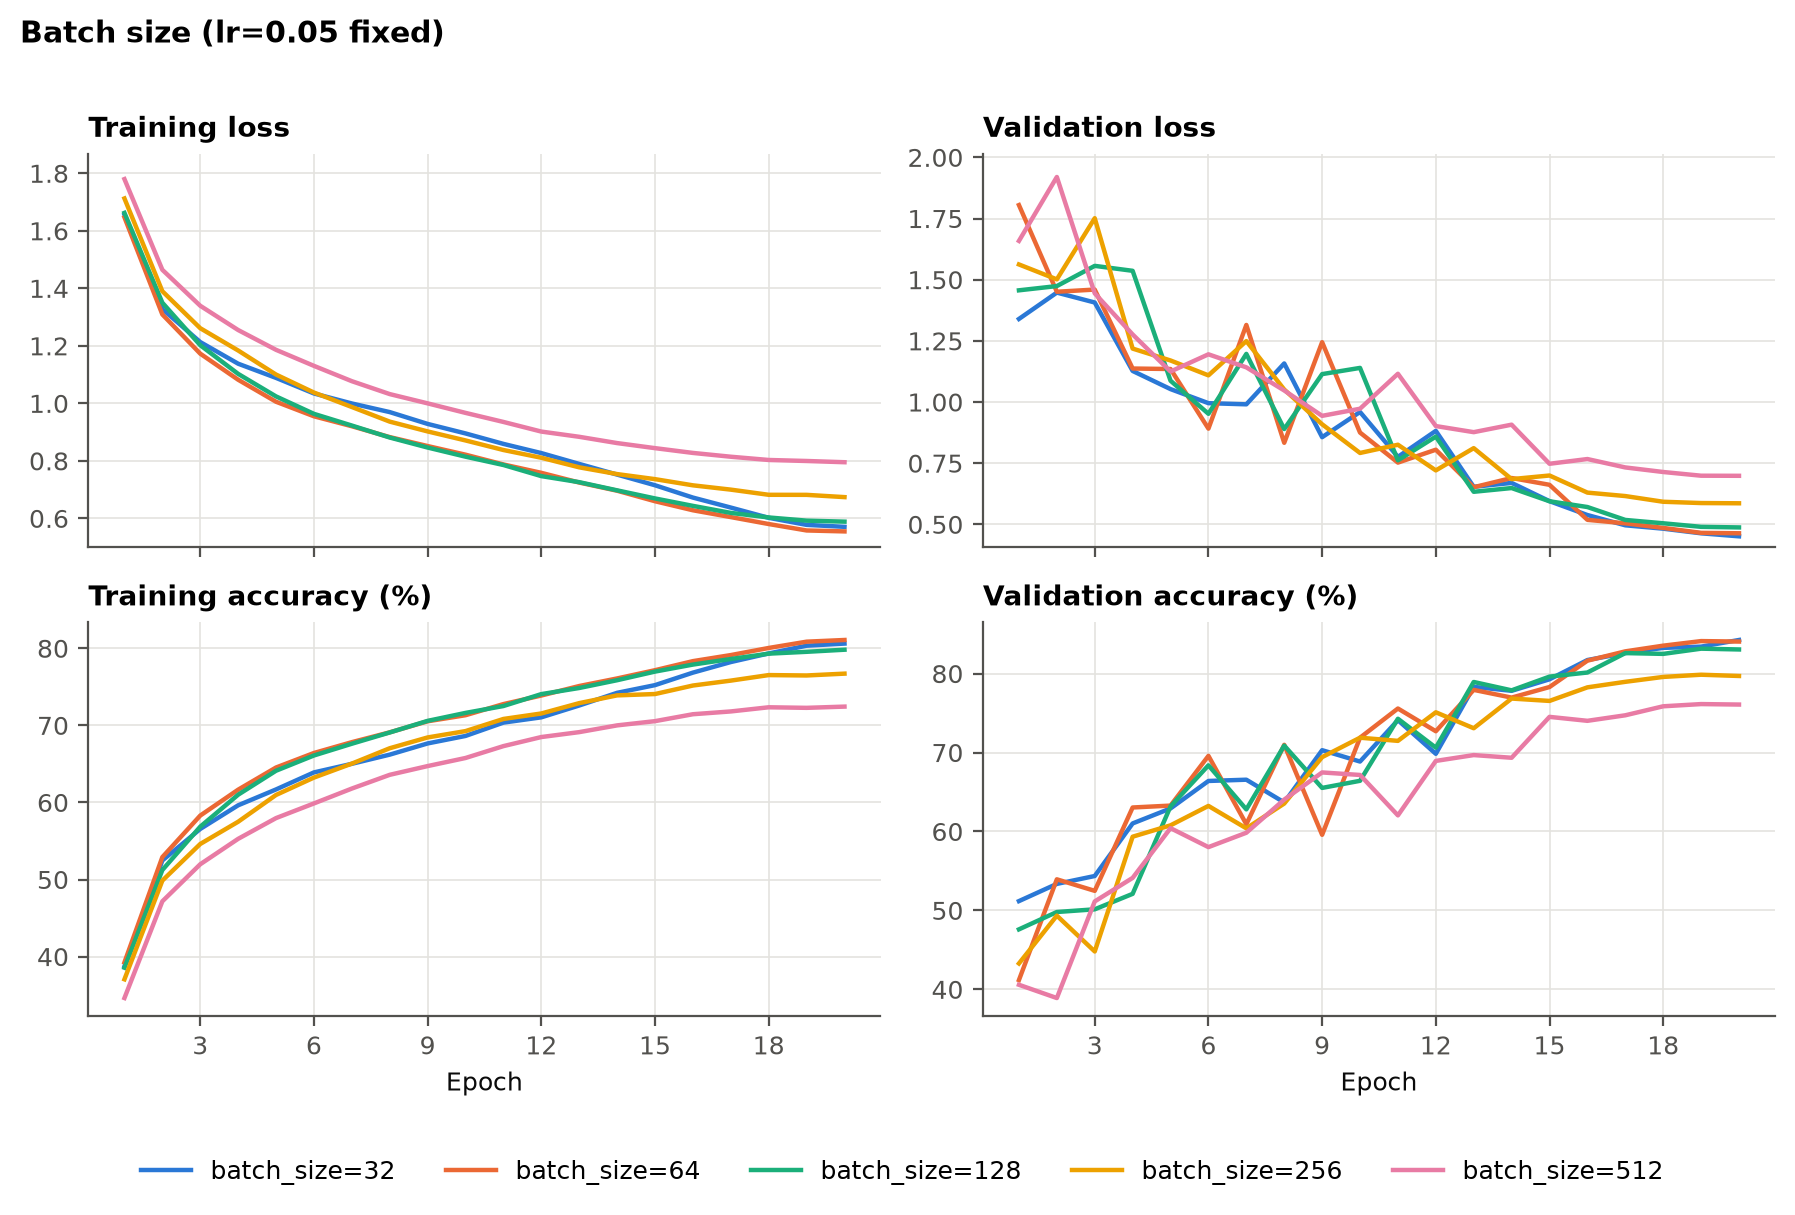
\includegraphics[width=0.78\linewidth]{figures/bs.png}
\caption{Batch size (lr 0.05, 20 epochs).}
\end{figure}
\begin{figure}[H]
\centering
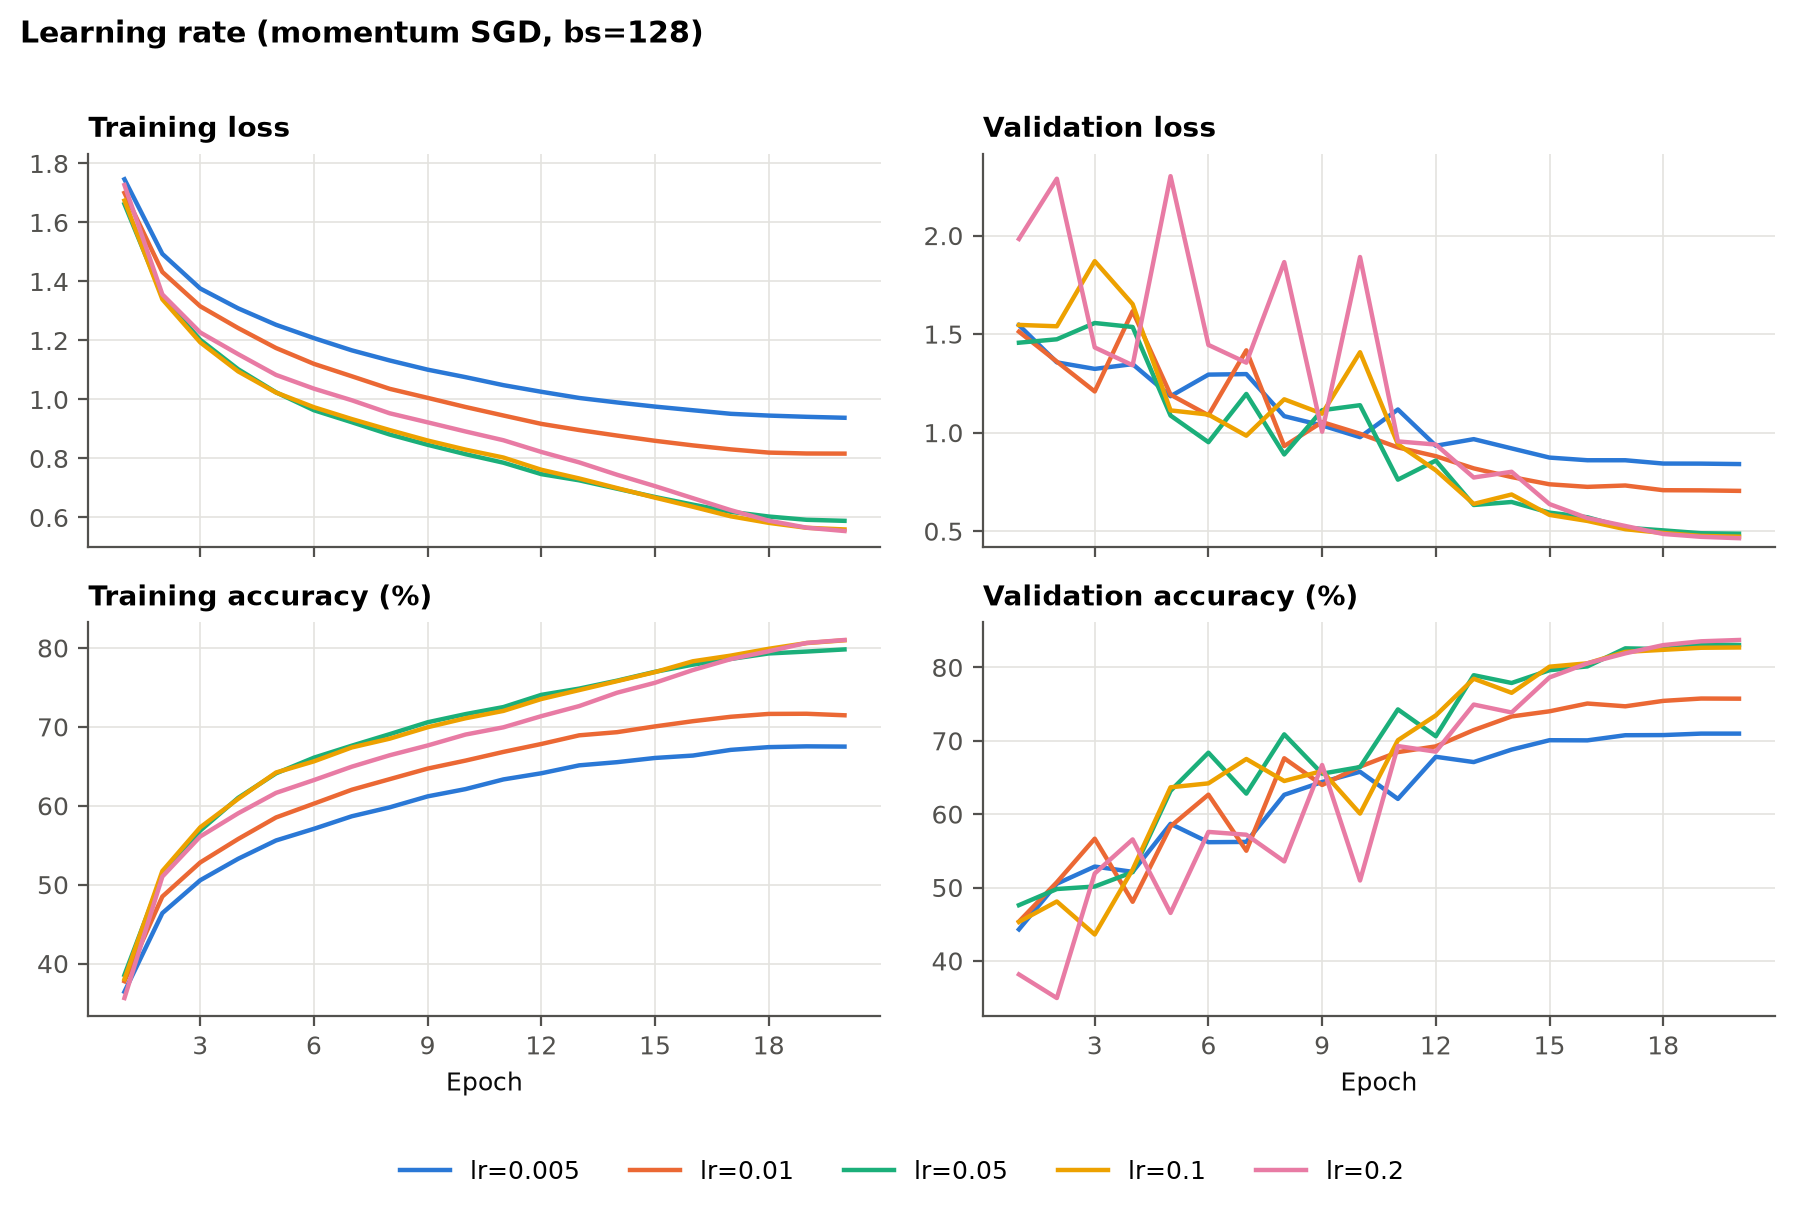
\includegraphics[width=0.78\linewidth]{figures/lr.png}
\caption{Learning rate (momentum SGD, batch 128, 20 epochs).}
\end{figure}
\begin{figure}[H]
\centering
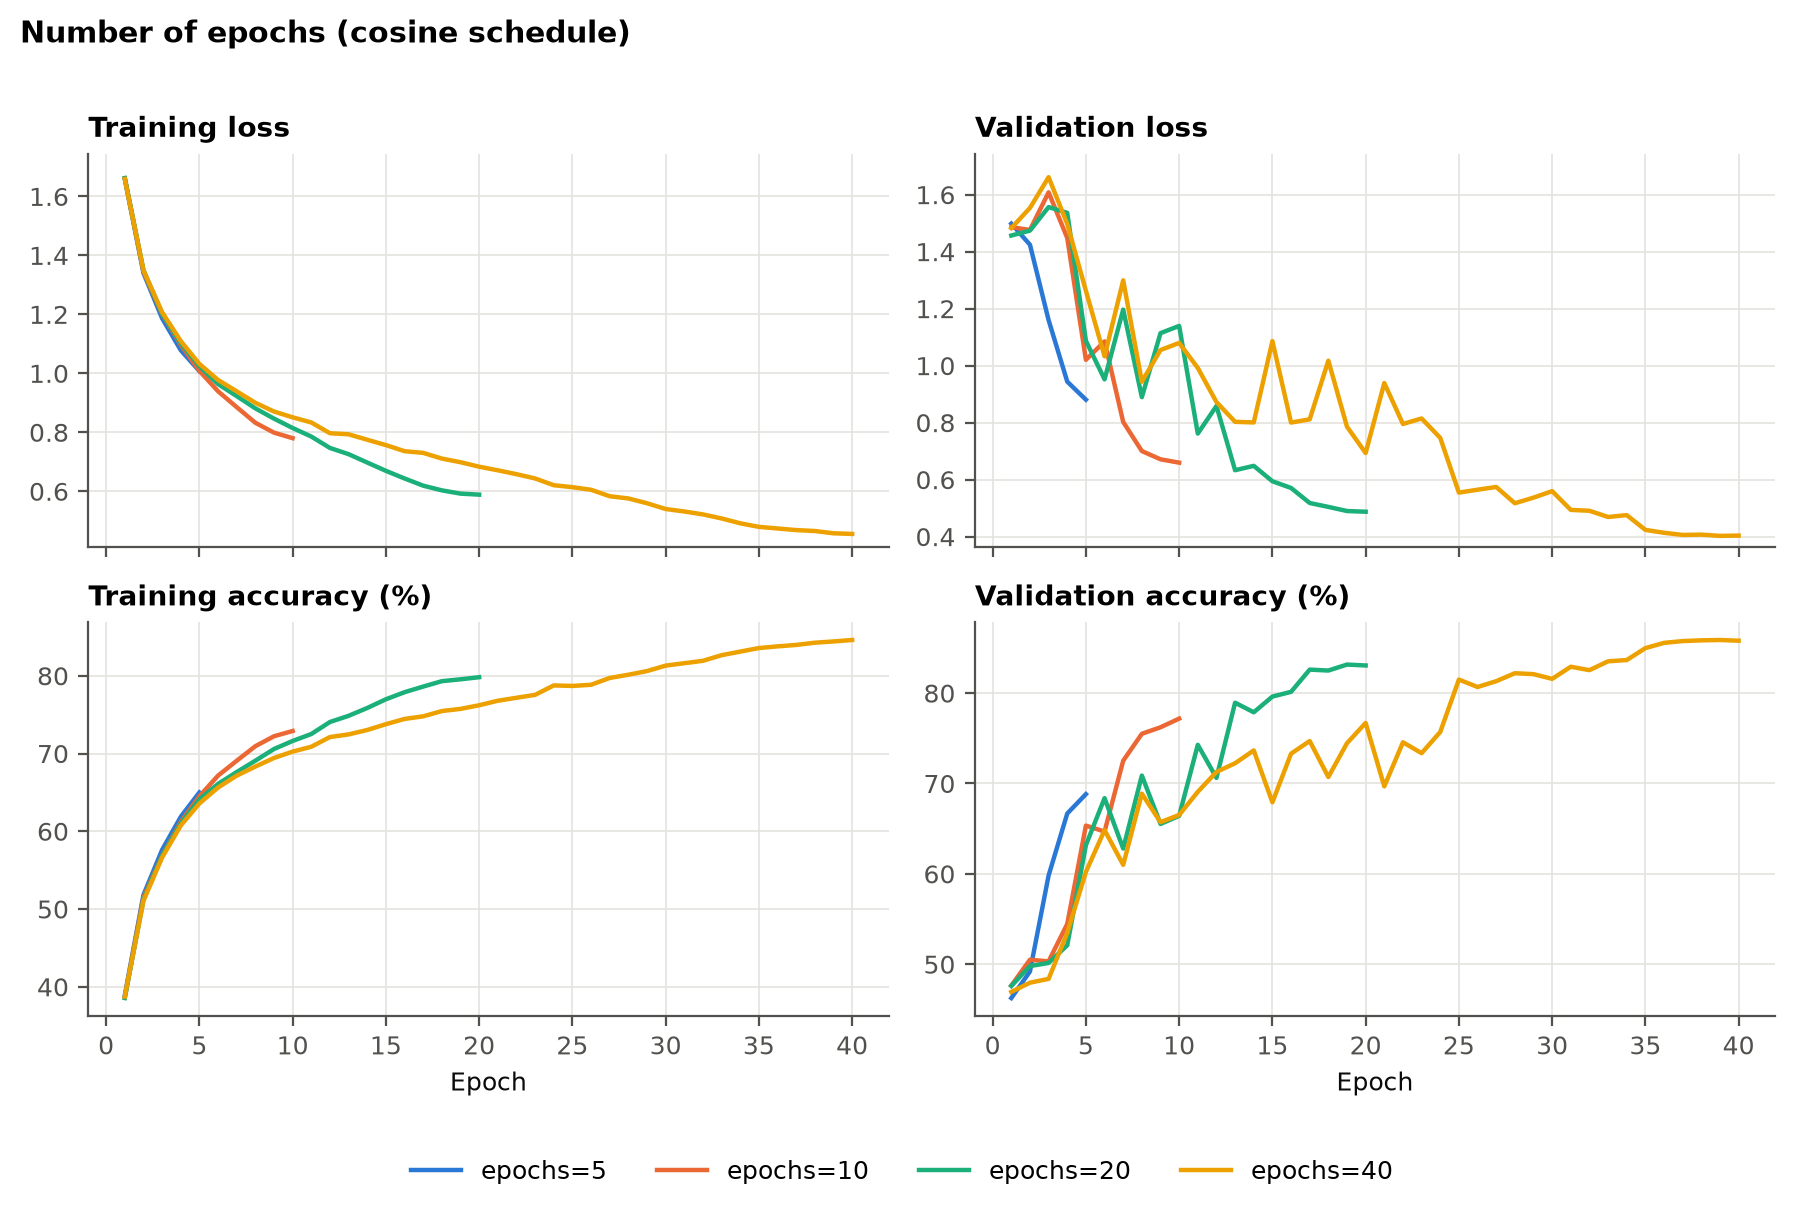
\includegraphics[width=0.78\linewidth]{figures/epochs.png}
\caption{Number of epochs (momentum SGD, lr 0.05, batch 128).}
\end{figure}

\textbf{Batch size.} With the learning rate and the number of epochs fixed, accuracy falls steadily as the batch grows: 84.3\% (32), 84.1\% (64), 83.2\% (128), 79.9\% (256), 76.1\% (512). The main reason is the number of parameter updates: one epoch is 1{,}407 steps at batch 32 but only 88 at batch 512, so after 20 epochs the large-batch model has taken 16$\times$ fewer steps of the same size and is still far from converged (70\% only at epoch 15 instead of 8 or 9). Small batches also add gradient noise, which helps escape sharp regions of the loss. The price is wall-clock time: the GPU is under-utilised by small batches, so an epoch takes 24.1\,s at batch 32 versus 17.2\,s at batch 512. Batch 64 is the best trade-off (84.1\% at 20.5\,s per epoch). Large batches are not inherently worse; they need a proportionally larger learning rate (linear scaling rule). The SGD noise scale is roughly proportional to lr/batch, and indeed batch 32 with lr 0.05 (84.3\%) and batch 128 with lr 0.2 (83.7\%), which have the same ratio, end almost equal.

\textbf{Learning rate.} Too small a learning rate converges slowly and is still under-trained after 20 epochs (71.0\% at 0.005, 75.8\% at 0.01; 70\% is reached only at epoch 15 and 13). From 0.05 to 0.2 the final accuracy plateaus at 82.7 to 83.7\%, differences within run-to-run noise. Larger rates make larger, noisier steps: with lr 0.2 the validation accuracy jumps by about 10 points from one epoch to the next during the first half (standard deviation of the epoch-to-epoch change 10.3 points, versus 5.2 at lr 0.05), and with lr 0.1 and 0.2 it reaches 70\% later (epochs 11 and 13) than with 0.05 (epoch 8). Both only catch up once the cosine schedule has lowered the rate. So a moderate learning rate gives the fastest early convergence, while somewhat larger ones explore more and finish equally well. BatchNorm makes the network unusually tolerant of large rates, because the convolution weights before a BatchNorm layer are scale-invariant, so a too-large step mainly increases the weight norm and thereby reduces the effective learning rate.

\textbf{Number of epochs.} More epochs help with diminishing returns: 68.8\% (5), 77.2\% (10), 83.2\% (20), 85.9\% (40), that is +8.4, +6.0 and +2.7 points per doubling. Because the cosine schedule is stretched over the run, a shorter run anneals sooner and reaches a given accuracy in fewer epochs (70\% at epoch 7 in the 10-epoch run versus epoch 8 in the 20-epoch run) but stops at a lower level. Training accuracy stays below validation accuracy even after 40 epochs, so the model is not over-fitting yet; this is why the final model is trained for 100 epochs. Cost grows linearly (about 18\,s per epoch).

\textbf{Summary.} Convergence speed per epoch is governed by the number of updates and their size (batch size and learning rate together, roughly through lr/batch), while the final accuracy is mainly limited by the total training budget (epochs) for this small, under-fitting network.

%=====================================================================
\section*{Question 3: Plots}

All plots below are produced automatically from the W\&B runs. The live versions are in the \wbreport{} of the W\&B project linked on the first page. The figures in this PDF are rendered from exactly the same logged per-epoch metrics by \texttt{scripts/make\_plots.py}, in the same layout as the W\&B panels (a W\&B screenshot saved as \texttt{report/figures/wandb/<panel>.png} replaces the corresponding rendering when the PDF is rebuilt).

\subsection*{(a) Parallel-coordinates plot}
\begin{figure}[H]
\centering
\wbfig{parallel_coordinates}{parallel_coordinates}{1.0}
\caption{Every run: hyper-parameters (axes) and best validation accuracy (colour, last axis).}
\end{figure}
\textbf{Reading the plot.} \ParallelDetail

\subsection*{(b) Validation accuracy vs.\ step (created)}
\begin{figure}[H]
\centering
\wbfig{valacc_scatter}{all_runs_valacc_scatter}{0.8}
\caption{Best validation accuracy of every run in order of creation; the line is the running maximum.}
\end{figure}

\subsection*{(c) Training loss, training accuracy, validation loss, validation accuracy}
\begin{figure}[H]
\centering
\wbfig{train_acc}{all_runs_train_acc}{0.49}\hfill
\wbfig{train_loss}{all_runs_train_loss}{0.49}\\[4pt]
\wbfig{val_acc}{all_runs_val_acc}{0.49}\hfill
\wbfig{val_loss}{all_runs_val_loss}{0.49}
\caption{train\_acc, train\_loss, val\_acc and val\_loss vs.\ epoch for all runs (colour = best validation accuracy of the run).}
\end{figure}

%=====================================================================
\section*{Question 4: Final model performance}

The run with the highest validation accuracy in the parallel-coordinates plot (Question 3a, top line of the last axis) is:

\begin{center}
\fbox{\parbox{0.9\linewidth}{\centering\small
\texttt{\BestName}\\[3pt]
activation = relu, batch\_norm = true, optimizer = nadam, lr = 0.003, weight\_decay = 0.0005,\\
batch\_size = 64, epochs = 100, scheduler = cosine, seed = 42\\
(momentum = 0.9 is in the config but unused by Nadam)\\[3pt]
\textbf{best validation accuracy \BestVal\%} (epoch \BestEpoch), \textbf{test accuracy \BestTest\%}}}
\end{center}

It is stored in \texttt{configs/best.yaml}, and the command in Question~5(c) reproduces it. The trained weights are \texttt{checkpoints/best\_model.pt}; \texttt{python evaluate.py} reloads them and prints the same validation and test accuracy. Reproducibility was checked in two ways: (1) re-evaluating the saved checkpoint gives exactly 86.36\% validation and 85.72\% test accuracy; (2) training \texttt{configs/best.yaml} twice from scratch (2 epochs) gave identical losses and accuracies to every printed digit, because all random numbers (initialisation, shuffling, augmentation) come from seeded generators. The per-class test accuracies of the final model range from 75.2\% (cat) and 78.5\% (dog) to 92.9\% (ship), so the two visually similar animal classes cat and dog are the hardest.

%=====================================================================
\section*{Question 5: Reproducibility and repository}

\textbf{(a) Code structure.} The code is split into a small package and thin entry scripts:
\begin{center}
\small
\begin{tabular}{ll}
\toprule
File & Responsibility \\
\midrule
\texttt{vgg6/data.py} & CIFAR-10 loading, 45k/5k split, normalisation and augmentation \\
\texttt{vgg6/model.py} & VGG6 with configurable activation and BatchNorm \\
\texttt{vgg6/optim.py} & optimizer and learning-rate schedule factories \\
\texttt{vgg6/engine.py} & \texttt{train\_one\_epoch}, \texttt{evaluate}, \texttt{predict} \\
\texttt{vgg6/utils.py} & seeding, device selection, run naming \\
\texttt{train.py} & training of one configuration, W\&B logging, checkpointing \\
\texttt{evaluate.py} & evaluation of a saved checkpoint (validation, test, per-class accuracy) \\
\texttt{run\_experiments.py} & the experiment families of Question 2 \\
\texttt{configs/best.yaml} & best configuration (Question 4) \\
\texttt{configs/sweep.yaml} & W\&B sweep definition \\
\texttt{scripts/make\_plots.py} & figures and tables of this PDF \\
\texttt{scripts/wandb\_report.py} & W\&B report with the Question 3 panels \\
\bottomrule
\end{tabular}
\end{center}

\textbf{(b) README.} The README lists the exact commands, the environment (macOS, Apple M1 Pro, Python 3.14.3, torch 2.14.1, torchvision 0.29.1, wandb 0.31.0, pinned in \texttt{requirements.txt}) and the seed configuration: seed 42 for Python, NumPy, PyTorch, batch shuffling and augmentation (a seeded CPU generator); the train/validation split uses its own fixed seed 0.

\textbf{(c) Trained model.} \texttt{checkpoints/best\_model.pt} (weights, configuration and metrics of the best run) is committed to the repository: \repo. Reproduce with
\begin{Verbatim}[frame=single,fontsize=\small]
python train.py --config configs/best.yaml
python evaluate.py --checkpoint checkpoints/best_model.pt
\end{Verbatim}

\end{document}
